%%This is a very basic article template.
%%There is just one section and two subsections.
\documentclass{report}

\usepackage{amssymb}
\usepackage{graphicx}
\usepackage{float}
\usepackage{color}
\usepackage{listings, multicol}
\usepackage{AMMALanguages}
%\usepackage{inconsolata}
\usepackage{url}
\usepackage{hyperref}
\usepackage{multirow}
\usepackage{etoolbox}
\usepackage{array}
\usepackage{multirow}
\usepackage{amsmath}
\usepackage{amssymb}
\usepackage{times}
\usepackage{changepage}
\usepackage{framed}
\usepackage{longtable}


\begin{document}

\title{Lazy OCL Performance Evaluation}

\part{Intro}

\chapter{Methodology}

In order to evaluate the gain in performance of the lazy evaluation
implementation of the OCL included in the EMFTVM w.r.t. a greedy evaluation
implementation we have conducted an experimental performance evaluation. It
consisted in testing, for each different collection type, the performance of
each collection and iteration operation and compare its time performance with
the time performance of the eager implementation of the standard ATL Virtual
Machine (ideally, an evaluation of the lazy OCL evaluation implementation of
EMFTVM against an eager implementation on the same VM would have been preferred,
but there is not such an eager implementation available).

\begin{figure*}[h]
\centering
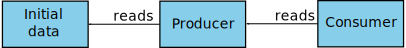
\includegraphics[width=10cm]{figures/producerConsumer}
\caption{Producer Consumer Schema}
\label{fig:producerConsumer}
\end{figure*}

The general schema for the evaluation of each operation follows a Producer
consumer pattern (see Figure \ref{fig:producerConsumer}) and is composed, as can
be seen in Figure \ref{fig:producerConsumerOCL} of three elements: 1) a source
collection, 2) the operation to test acting as a value producer, and 3) a
consumer that will incrementally (when it applies) request that values generated
by the producer from the source collection.

\begin{figure*}[h]
\centering
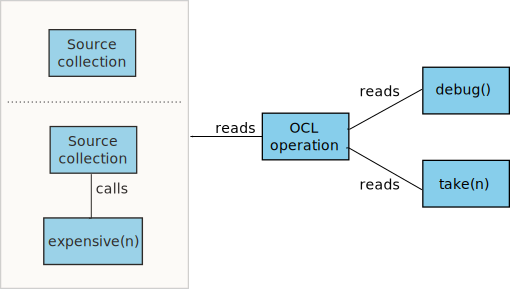
\includegraphics[width=10cm]{figures/producerConsumerOCL}
\caption{Producer Consumer Instantiated for OCL evaluation}
\label{fig:producerConsumerOCL}
\end{figure*}

We also provide an especial operation, \emph{expensive()}, intended to
add computation complexity to the evaluation process without requiring too large
collections. We have decided to implement a product of a recursive factorial as
our \emph{expensive()} operation. We use the product operation in
order to increment the evaluation time for the operation while avoiding the 
exhaustion of the memory heap due to the recursive calls. Note that for the
purpose of this experimentation, we are not interested in the returned value of
this operation. We will consider it to return 0 as it is the case for any
factorial input value greater than 10 due to the overflow of the Integer
representation (if used with smaller values of factorial, the expensive
operation would need to be refactored to return 0 as other values may distort
the results of the tests).

\begin{lstlisting}[language=ATL, style=AMMA,
label=lst:expensiveOP, caption=expensive() operation] 

helper context Integer def : expensive() : Integer =
	thisModule.factorial(thisModule.expensiveValue)*thisModule.factorial(thisModule.expensiveValue);
		

helper def : factorial(val: Integer) : Integer =
	if(val = 1) then 
		1
	else
		val * thisModule.factorial(val-1)
	endif;

\end{lstlisting}


We provide two source collections. \emph{Numbers(end: Integer)} and
\emph{Squares(end:Integer)}. As can be seen in Listings \ref{lst:NumbersOP} and
\ref{lst:SquaresOP} they basically take an EMF collection from a model passed as
parameter (namely, a list of numbers called 'Naturals' with natural numbers from
0 to 750 and a lisf of numbers called 'Sqaures' with the squares of numbers
between 0 and 750) to the transformation model and return a sub-collection of
numbers from 1 to end and a sub-collection of squares from 1 to end. Note that
all the operations we present here operates on a concrete collection type are
thus, we have to refactor these two operations to work with the other collection
types in the corresponding tests by using the asSet(), asBag() and as
asOrderedSet() operations.

\begin{lstlisting}[language=ATL, style=AMMA,
label=lst:NumbersOP, caption=Numbers() operation] 

helper def : Numbers(end: Integer) : Sequence(Integer) =
	Parameters!Parameter.allInstances()
	->select(e|e.name = 'Naturals')
	->first().list->subSequence(1,end);


\end{lstlisting}

\begin{lstlisting}[language=ATL, style=AMMA,
label=lst:SquaresOP, caption=Squares() operation]
 
helper def : squares(end: Integer) : Sequence(Integer) =
	Parameters!Parameter.allInstances()
	->select(e|e.name = 'Squares')
	->first().list->subSequence(1,end);

\end{lstlisting}

Our consumer, for operations returning a collection is as shown in listing
\ref{lst:takeOP}. For operations returning single values, we will use the greedy
operation \emph{debug()} that prints in console the result of a given operation
and thus, makes sure the calculation is performed.

The \emph{take(n:Integer, col: Collection(Integer))} operation recursively
builds a collection by taking N elements from the input collection. This
simulates the iterative consumption of the source collection (to which we have
applied the operation to be tested) allowing us to evaluate the performance of
the lazy calculation evaluation for different values of N.

\begin{lstlisting}[language=ATL, style=AMMA,
label=lst:takeOP, caption=take() operation] 

helper def: take(n: Integer, seq: Sequence(Integer)) : Sequence(Integer) = 
	if(n = 1) then
		Sequence{1}
	else
		let prev:Sequence(Integer) = thisModule.take(n-1, seq) in
			prev->including(seq->any(x|prev->excludes(x)))
	endif;


-- Alternative implementation with collection as context
helper context Sequence(Integer) def : takeFromSeq(n:Integer):Sequence(Integer) = 
	if(n = 1) then
		Sequence{1}
	else
		let prev:Sequence(Integer) = self.takeFromSeq(n-1) in
			prev->including(self->any(x|prev->excludes(x)))
	endif;

\end{lstlisting}

\section{Non available operations}

Some operations could have not been tested because they are not available in the
implementation of at least one of the VMs. In the following we will list all the
missing operations.

\subsection{Sequence}

\begin{itemize}
  \item Max()
  \item Reverse()
  \item CollectNested()
\end{itemize}

\subsection{Set}

\begin{itemize}
  \item Reverse()
\end{itemize}

\subsection{Bag}

\begin{itemize}
  \item Intersection()
  \item SymmetricDifference()
  \item Minus()
\end{itemize}

\subsection{OrderedSet}
 
 Operations not available in the standard VM

\begin{itemize}
  \item At() (OrderedSet is implemented as a LinkedHashSet that does not
  provide a get operation, preventing an easy an efficient implementation of at())
  \item Max()
  \item Reverse()
\end{itemize}




\part{Performance Evaluation Results}

We will present the evaluation results for each of the OCL operations separated
by collection type.

\chapter{Sequence}


\noindent\textbf{Any}
\lstinputlisting[firstline=1,lastline=3]{transformations/sequence/emftvm/TestAny.atl}
\begin{figure*}[h]
\centering	
\includegraphics[width=\textwidth]{graphs/sequence/Any}
\end{figure*}
\pagebreak

\noindent\textbf{Append}
\lstinputlisting[firstline=1,lastline=3]{transformations/sequence/emftvm/TestAppend.atl}
\begin{figure*}[h]
\centering
\includegraphics[width=\textwidth]{graphs/sequence/Append}
\end{figure*}
\pagebreak

\noindent\textbf{At}
\lstinputlisting[firstline=1,lastline=3]{transformations/sequence/emftvm/TestAt.atl}
\begin{figure*}[h]
\centering
\includegraphics[width=\textwidth]{graphs/sequence/At}
\end{figure*}
\pagebreak

\noindent\textbf{Collect}
\lstinputlisting[firstline=1,lastline=3]{transformations/sequence/emftvm/TestCollect.atl}
\begin{figure*}[h]
\centering
\includegraphics[width=\textwidth]{graphs/sequence/Collect}
\end{figure*}
\pagebreak

\noindent\textbf{EQ}
\lstinputlisting[firstline=1,lastline=3]{transformations/sequence/emftvm/TestEQ.atl}
\begin{figure*}[h]
\centering
\includegraphics[width=\textwidth]{graphs/sequence/EQ}
\end{figure*}
\pagebreak

\noindent\textbf{Excludes}
\lstinputlisting[firstline=1,lastline=3]{transformations/sequence/emftvm/TestExcludes.atl}
\begin{figure*}[h]
\centering
\includegraphics[width=\textwidth]{graphs/sequence/Excludes}
\end{figure*}
\pagebreak

\noindent\textbf{ExcludesAll}
\lstinputlisting[firstline=1,lastline=3]{transformations/sequence/emftvm/TestExcludesAll.atl}
\begin{figure*}[h]
\centering
\includegraphics[width=\textwidth]{graphs/sequence/ExcludesAll}
\end{figure*}
\pagebreak

\noindent\textbf{Excluding}
\lstinputlisting[firstline=1,lastline=3]{transformations/sequence/emftvm/TestExcluding.atl}
\begin{figure*}[h]
\centering
\includegraphics[width=\textwidth]{graphs/sequence/Excluding}
\end{figure*}
\pagebreak

\noindent\textbf{Exists}
\lstinputlisting[firstline=1,lastline=3]{transformations/sequence/emftvm/TestExists.atl}
\begin{figure*}[h]
\centering
\includegraphics[width=\textwidth]{graphs/sequence/Exists}
\end{figure*}
\pagebreak

\noindent\textbf{First}
\lstinputlisting[firstline=1,lastline=3]{transformations/sequence/emftvm/TestFirst.atl}
\begin{figure*}[h]
\centering
\includegraphics[width=\textwidth]{graphs/sequence/First}
\end{figure*}
\pagebreak

\noindent\textbf{Flatten}
\lstinputlisting[firstline=1,lastline=3]{transformations/sequence/emftvm/TestFlatten.atl}
\begin{figure*}[h]
\centering
\includegraphics[width=\textwidth]{graphs/sequence/Flatten}
\end{figure*}
\pagebreak

\noindent\textbf{ForAll}
\lstinputlisting[firstline=1,lastline=3]{transformations/sequence/emftvm/TestForAll.atl}
\begin{figure*}[h]
\centering
\includegraphics[width=\textwidth]{graphs/sequence/forALL}
\end{figure*}
\pagebreak

\noindent\textbf{Includes}
\lstinputlisting[firstline=1,lastline=3]{transformations/sequence/emftvm/TestIncludes.atl}
\begin{figure*}[h]
\centering
\includegraphics[width=\textwidth]{graphs/sequence/Includes}
\end{figure*}
\pagebreak

\noindent\textbf{IncludesAll}
\lstinputlisting[firstline=1,lastline=3]{transformations/sequence/emftvm/TestIncludesAll.atl}
\begin{figure*}[h]
\centering
\includegraphics[width=\textwidth]{graphs/sequence/IncludesAll}
\end{figure*}
\pagebreak

\noindent\textbf{Including}
\lstinputlisting[firstline=1,lastline=3]{transformations/sequence/emftvm/TestIncluding.atl}
\begin{figure*}[h]
\centering
\includegraphics[width=\textwidth]{graphs/sequence/Including}
\end{figure*}
\pagebreak

\noindent\textbf{IndexOf}
\lstinputlisting[firstline=1,lastline=3]{transformations/sequence/emftvm/TestIndexOf.atl}
\begin{figure*}[h]
\centering
\includegraphics[width=\textwidth]{graphs/sequence/IndexOf}
\end{figure*}
\pagebreak

\noindent\textbf{InsertAt}
\lstinputlisting[firstline=1,lastline=3]{transformations/sequence/emftvm/TestInsertAt.atl}
\begin{figure*}[h]
\centering
\includegraphics[width=\textwidth]{graphs/sequence/InsertAt}
\end{figure*}
\pagebreak

\noindent\textbf{IsEmpty}
\lstinputlisting[firstline=1,lastline=3]{transformations/sequence/emftvm/TestIsEmpty.atl}
\begin{figure*}[h]
\centering
\includegraphics[width=\textwidth]{graphs/sequence/IsEmpty}
\end{figure*}
\pagebreak

\noindent\textbf{IsUnique}
\lstinputlisting[firstline=1,lastline=3]{transformations/sequence/emftvm/TestIsUnique.atl}
\begin{figure*}[h]
\centering
\includegraphics[width=\textwidth]{graphs/sequence/isUnique}
\end{figure*}
\pagebreak

\noindent\textbf{Iterate}
\lstinputlisting[firstline=1,lastline=3]{transformations/sequence/emftvm/TestIterate.atl}
\begin{figure*}[h]
\centering
\includegraphics[width=\textwidth]{graphs/sequence/Iterate}
\end{figure*}
\pagebreak

\noindent\textbf{Last}
\lstinputlisting[firstline=1,lastline=3]{transformations/sequence/emftvm/TestLast.atl}
\begin{figure*}[h]
\centering
\includegraphics[width=\textwidth]{graphs/sequence/Last}
\end{figure*}
\pagebreak

\noindent\textbf{NotEqual}
\lstinputlisting[firstline=1,lastline=3]{transformations/sequence/emftvm/TestNeq.atl}
\begin{figure*}[h]
\centering
\includegraphics[width=\textwidth]{graphs/sequence/NEQ}
\end{figure*}
\pagebreak

\noindent\textbf{One}
\lstinputlisting[firstline=1,lastline=3]{transformations/sequence/emftvm/TestOne.atl}
\begin{figure*}[h]
\centering
\includegraphics[width=\textwidth]{graphs/sequence/One}
\end{figure*}
\pagebreak

\noindent\textbf{Prepend}
\lstinputlisting[firstline=1,lastline=3]{transformations/sequence/emftvm/TestPrepend.atl}
\begin{figure*}[h]
\centering
\includegraphics[width=\textwidth]{graphs/sequence/Prepend}
\end{figure*}
\pagebreak

\noindent\textbf{Reject}
\lstinputlisting[firstline=1,lastline=3]{transformations/sequence/emftvm/TestReject.atl}
\begin{figure*}[h]
\centering
\includegraphics[width=\textwidth]{graphs/sequence/Reject}
\end{figure*}
\pagebreak

\noindent\textbf{Select}
\lstinputlisting[firstline=1,lastline=3]{transformations/sequence/emftvm/TestSelect.atl}
\begin{figure*}[h]
\centering
\includegraphics[width=\textwidth]{graphs/sequence/Select}
\end{figure*}
\pagebreak

\noindent\textbf{Size}
\lstinputlisting[firstline=1,lastline=3]{transformations/sequence/emftvm/TestSize.atl}
\begin{figure*}[h]
\centering
\includegraphics[width=\textwidth]{graphs/sequence/Size}
\end{figure*}
\pagebreak

\noindent\textbf{SortedBy}
\lstinputlisting[firstline=1,lastline=3]{transformations/sequence/emftvm/TestSortedBy.atl}
\begin{figure*}[h]
\centering
\includegraphics[width=\textwidth]{graphs/sequence/sortedBy}
\end{figure*}
\pagebreak

\noindent\textbf{SubSequence}
\lstinputlisting[firstline=1,lastline=3]{transformations/sequence/emftvm/TestSubsequence.atl}
\begin{figure*}[h]
\centering
\includegraphics[width=\textwidth]{graphs/sequence/SubSequence}
\end{figure*}
\pagebreak

\noindent\textbf{Sum}
\lstinputlisting[firstline=1,lastline=3]{transformations/sequence/emftvm/TestSum.atl}
\begin{figure*}[h]
\centering
\includegraphics[width=\textwidth]{graphs/sequence/Sum}
\end{figure*}
\pagebreak

\noindent\textbf{Union}
\lstinputlisting[firstline=1,lastline=3]{transformations/sequence/emftvm/TestUnion.atl}
\begin{figure*}[h]
\centering
\includegraphics[width=\textwidth]{graphs/sequence/Union}
\end{figure*}
\pagebreak

\chapter{Set}

\noindent\textbf{Any}
\lstinputlisting[firstline=1,lastline=3]{../transformations/set/emftvm/TestAny.atl}
\begin{figure*}[h]
\centering
\includegraphics[width=\textwidth]{../graphs/set/Any}
\end{figure*}
\pagebreak

\noindent\textbf{Collect}
\lstinputlisting[firstline=1,lastline=3]{../transformations/set/emftvm/TestCollect.atl}
\begin{figure*}[h]
\centering
\includegraphics[width=\textwidth]{../graphs/set/Collect}
\end{figure*}
\pagebreak

\noindent\textbf{EQ}
\lstinputlisting[firstline=1,lastline=3]{../transformations/set/emftvm/TestEQ.atl}
\begin{figure*}[h]
\centering
\includegraphics[width=\textwidth]{../graphs/set/EQ}
\end{figure*}
\pagebreak

\noindent\textbf{Excludes}
\lstinputlisting[firstline=1,lastline=3]{../transformations/set/emftvm/TestExcludes.atl}
\begin{figure*}[h]
\centering
\includegraphics[width=\textwidth]{../graphs/set/Excludes}
\end{figure*}
\pagebreak

\noindent\textbf{ExcludesAll}
\lstinputlisting[firstline=1,lastline=3]{../transformations/set/emftvm/TestExcludesAll.atl}
\begin{figure*}[h]
\centering
\includegraphics[width=\textwidth]{../graphs/set/ExcludesAll}
\end{figure*}
\pagebreak

\noindent\textbf{Excluding}
\lstinputlisting[firstline=1,lastline=3]{../transformations/set/emftvm/TestExcluding.atl}
\begin{figure*}[h]
\centering
\includegraphics[width=\textwidth]{../graphs/set/Excluding}
\end{figure*}
\pagebreak

\noindent\textbf{Exists}
\lstinputlisting[firstline=1,lastline=3]{../transformations/set/emftvm/TestExists.atl}
\begin{figure*}[h]
\centering
\includegraphics[width=\textwidth]{../graphs/set/Exists}
\end{figure*}
\pagebreak

\noindent\textbf{Flatten}
\lstinputlisting[firstline=1,lastline=3]{../transformations/set/emftvm/TestFlatten.atl}
\begin{figure*}[h]
\centering
\includegraphics[width=\textwidth]{../graphs/set/Flatten}
\end{figure*}
\pagebreak

\noindent\textbf{ForAll}
\lstinputlisting[firstline=1,lastline=3]{../transformations/set/emftvm/TestForAll.atl}
\begin{figure*}[h]
\centering
\includegraphics[width=\textwidth]{../graphs/set/forALL}
\end{figure*}
\pagebreak

\noindent\textbf{Includes}
\lstinputlisting[firstline=1,lastline=3]{../transformations/set/emftvm/TestIncludes.atl}
\begin{figure*}[h]
\centering
\includegraphics[width=\textwidth]{../graphs/set/Includes}
\end{figure*}
\pagebreak

\noindent\textbf{IncludesAll}
\lstinputlisting[firstline=1,lastline=3]{../transformations/set/emftvm/TestIncludesAll.atl}
\begin{figure*}[h]
\centering
\includegraphics[width=\textwidth]{../graphs/set/IncludesAll}
\end{figure*}
\pagebreak

\noindent\textbf{Including}
\lstinputlisting[firstline=1,lastline=3]{../transformations/set/emftvm/TestIncluding.atl}
\begin{figure*}[h]
\centering
\includegraphics[width=\textwidth]{../graphs/set/Including}
\end{figure*}
\pagebreak

\noindent\textbf{Intersection}
\lstinputlisting[firstline=1,lastline=3]{../transformations/set/emftvm/TestIntersection.atl}
\begin{figure*}[h]
\centering
\includegraphics[width=\textwidth]{../graphs/set/Intersection}
\end{figure*}
\pagebreak

\noindent\textbf{IsEmpty}
\lstinputlisting[firstline=1,lastline=3]{../transformations/set/emftvm/TestIsEmpty.atl}
\begin{figure*}[h]
\centering
\includegraphics[width=\textwidth]{../graphs/set/IsEmpty}
\end{figure*}
\pagebreak

\noindent\textbf{IsUnique}
\lstinputlisting[firstline=1,lastline=3]{../transformations/set/emftvm/TestIsUnique.atl}
\begin{figure*}[h]
\centering
\includegraphics[width=\textwidth]{../graphs/set/isUnique}
\end{figure*}
\pagebreak

\noindent\textbf{Iterate}
\lstinputlisting[firstline=1,lastline=3]{../transformations/set/emftvm/TestIterate.atl}
\begin{figure*}[h]
\centering
\includegraphics[width=\textwidth]{../graphs/set/Iterate}
\end{figure*}
\pagebreak

\noindent\textbf{Minus}
\lstinputlisting[firstline=1,lastline=3]{../transformations/set/emftvm/TestMinus.atl}
\begin{figure*}[h]
\centering
\includegraphics[width=\textwidth]{../graphs/set/Minus}
\end{figure*}
\pagebreak

\noindent\textbf{NotEqual}
\lstinputlisting[firstline=1,lastline=3]{../transformations/set/emftvm/TestNeq.atl}
\begin{figure*}[h]
\centering
\includegraphics[width=\textwidth]{../graphs/set/NEQ}
\end{figure*}
\pagebreak

\noindent\textbf{One}
\lstinputlisting[firstline=1,lastline=3]{../transformations/set/emftvm/TestOne.atl}
\begin{figure*}[h]
\centering
\includegraphics[width=\textwidth]{../graphs/set/One}
\end{figure*}
\pagebreak

\noindent\textbf{Reject}
\lstinputlisting[firstline=1,lastline=3]{../transformations/set/emftvm/TestReject.atl}
\begin{figure*}[h]
\centering
\includegraphics[width=\textwidth]{../graphs/set/Reject}
\end{figure*}
\pagebreak

\noindent\textbf{Select}
\lstinputlisting[firstline=1,lastline=3]{../transformations/set/emftvm/TestSelect.atl}
\begin{figure*}[h]
\centering
\includegraphics[width=\textwidth]{../graphs/set/Select}
\end{figure*}
\pagebreak

\noindent\textbf{Size}
\lstinputlisting[firstline=1,lastline=3]{../transformations/set/emftvm/TestSize.atl}
\begin{figure*}[h]
\centering
\includegraphics[width=\textwidth]{../graphs/set/Size}
\end{figure*}
\pagebreak

\noindent\textbf{SortedBy}
\lstinputlisting[firstline=1,lastline=3]{../transformations/set/emftvm/TestSortedBy.atl}
\begin{figure*}[h]
\centering
\includegraphics[width=\textwidth]{../graphs/set/sortedBy}
\end{figure*}
\pagebreak

\noindent\textbf{Sum}
\lstinputlisting[firstline=1,lastline=3]{../transformations/set/emftvm/TestSum.atl}
\begin{figure*}[h]
\centering
\includegraphics[width=\textwidth]{../graphs/set/Sum}
\end{figure*}
\pagebreak

\noindent\textbf{SymmetricDif}
\lstinputlisting[firstline=1,lastline=3]{../transformations/set/emftvm/TestSymmetricDif.atl}
\begin{figure*}[h]
\centering
\includegraphics[width=\textwidth]{../graphs/set/SymmetricDif}
\end{figure*}
\pagebreak

\noindent\textbf{Union}
\lstinputlisting[firstline=1,lastline=3]{../transformations/set/emftvm/TestUnion.atl}
\begin{figure*}[h]
\centering
\includegraphics[width=\textwidth]{../graphs/set/Union}
\end{figure*}
\pagebreak

\chapter{Bag}

\noindent\textbf{Any}
\lstinputlisting[firstline=1,lastline=3]{transformations/bag/emftvm/TestAny.atl}
\begin{figure*}[h]
\centering
\includegraphics[width=\textwidth]{graphs/bag/Any}
\end{figure*}
\pagebreak

\noindent\textbf{Collect}
\lstinputlisting[firstline=1,lastline=3]{transformations/bag/emftvm/TestCollect.atl}
\begin{figure*}[h]
\centering
\includegraphics[width=\textwidth]{graphs/bag/Collect}
\end{figure*}
\pagebreak

\noindent\textbf{EQ}
\lstinputlisting[firstline=1,lastline=3]{transformations/bag/emftvm/TestEQ.atl}
\begin{figure*}[h]
\centering
\includegraphics[width=\textwidth]{graphs/bag/EQ}
\end{figure*}
\pagebreak

\noindent\textbf{Excludes}
\lstinputlisting[firstline=1,lastline=3]{transformations/bag/emftvm/TestExcludes.atl}
\begin{figure*}[h]
\centering
\includegraphics[width=\textwidth]{graphs/bag/Excludes}
\end{figure*}
\pagebreak

\noindent\textbf{ExcludesAll}
\lstinputlisting[firstline=1,lastline=3]{transformations/bag/emftvm/TestExcludesAll.atl}
\begin{figure*}[h]
\centering
\includegraphics[width=\textwidth]{graphs/bag/ExcludesAll}
\end{figure*}
\pagebreak

\noindent\textbf{Excluding}
\lstinputlisting[firstline=1,lastline=3]{transformations/bag/emftvm/TestExcluding.atl}
\begin{figure*}[h]
\centering
\includegraphics[width=\textwidth]{graphs/bag/Excluding}
\end{figure*}
\pagebreak

\noindent\textbf{Exists}
\lstinputlisting[firstline=1,lastline=3]{transformations/bag/emftvm/TestExists.atl}
\begin{figure*}[h]
\centering
\includegraphics[width=\textwidth]{graphs/bag/Exists}
\end{figure*}
\pagebreak

\noindent\textbf{Flatten}
\lstinputlisting[firstline=1,lastline=3]{transformations/bag/emftvm/TestFlatten.atl}
\begin{figure*}[h]
\centering
\includegraphics[width=\textwidth]{graphs/bag/Flatten}
\end{figure*}
\pagebreak

\noindent\textbf{ForAll}
\lstinputlisting[firstline=1,lastline=3]{transformations/bag/emftvm/TestForAll.atl}
\begin{figure*}[h]
\centering
\includegraphics[width=\textwidth]{graphs/bag/forALL}
\end{figure*}
\pagebreak

\noindent\textbf{Includes}
\lstinputlisting[firstline=1,lastline=3]{transformations/bag/emftvm/TestIncludes.atl}
\begin{figure*}[h]
\centering
\includegraphics[width=\textwidth]{graphs/bag/Includes}
\end{figure*}
\pagebreak

\noindent\textbf{IncludesAll}
\lstinputlisting[firstline=1,lastline=3]{transformations/bag/emftvm/TestIncludesAll.atl}
\begin{figure*}[h]
\centering
\includegraphics[width=\textwidth]{graphs/bag/IncludesAll}
\end{figure*}
\pagebreak

\noindent\textbf{Including}
\lstinputlisting[firstline=1,lastline=3]{transformations/bag/emftvm/TestIncluding.atl}
\begin{figure*}[h]
\centering
\includegraphics[width=\textwidth]{graphs/bag/Including}
\end{figure*}
\pagebreak

\noindent\textbf{IsEmpty}
\lstinputlisting[firstline=1,lastline=3]{transformations/bag/emftvm/TestIsEmpty.atl}
\begin{figure*}[h]
\centering
\includegraphics[width=\textwidth]{graphs/bag/IsEmpty}
\end{figure*}
\pagebreak

\noindent\textbf{IsUnique}
\lstinputlisting[firstline=1,lastline=3]{transformations/bag/emftvm/TestIsUnique.atl}
\begin{figure*}[h]
\centering
\includegraphics[width=\textwidth]{graphs/bag/isUnique}
\end{figure*}
\pagebreak

\noindent\textbf{Iterate}
\lstinputlisting[firstline=1,lastline=3]{transformations/bag/emftvm/TestIterate.atl}
\begin{figure*}[h]
\centering
\includegraphics[width=\textwidth]{graphs/bag/Iterate}
\end{figure*}
\pagebreak

\noindent\textbf{NotEqual}
\lstinputlisting[firstline=1,lastline=3]{transformations/bag/emftvm/TestNeq.atl}
\begin{figure*}[h]
\centering
\includegraphics[width=\textwidth]{graphs/bag/NEQ}
\end{figure*}
\pagebreak

\noindent\textbf{One}
\lstinputlisting[firstline=1,lastline=3]{transformations/bag/emftvm/TestOne.atl}
\begin{figure*}[h]
\centering
\includegraphics[width=\textwidth]{graphs/bag/One}
\end{figure*}
\pagebreak

\noindent\textbf{Reject}
\lstinputlisting[firstline=1,lastline=3]{transformations/bag/emftvm/TestReject.atl}
\begin{figure*}[h]
\centering
\includegraphics[width=\textwidth]{graphs/bag/Reject}
\end{figure*}
\pagebreak

\noindent\textbf{Select}
\lstinputlisting[firstline=1,lastline=3]{transformations/bag/emftvm/TestSelect.atl}
\begin{figure*}[h]
\centering
\includegraphics[width=\textwidth]{graphs/bag/Select}
\end{figure*}
\pagebreak

\noindent\textbf{Size}
\lstinputlisting[firstline=1,lastline=3]{transformations/bag/emftvm/TestSize.atl}
\begin{figure*}[h]
\centering
\includegraphics[width=\textwidth]{graphs/bag/Size}
\end{figure*}
\pagebreak

\noindent\textbf{SortedBy}
\lstinputlisting[firstline=1,lastline=3]{transformations/bag/emftvm/TestSortedBy.atl}
\begin{figure*}[h]
\centering
\includegraphics[width=\textwidth]{graphs/bag/sortedBy}
\end{figure*}e
\pagebreak

\noindent\textbf{Sum}
\lstinputlisting[firstline=1,lastline=3]{transformations/bag/emftvm/TestSum.atl}
\begin{figure*}[h]
\centering
\includegraphics[width=\textwidth]{graphs/bag/Sum}
\end{figure*}
\pagebreak


\chapter{OrderedSet}

\noindent\textbf{Any}
\lstinputlisting[firstline=1,lastline=3]{../transformations/orderedset/emftvm/TestAny.atl}
\begin{figure*}[h]
\centering
\includegraphics[width=\textwidth]{../graphs/orderedset/Any}
\end{figure*}
\pagebreak

\noindent\textbf{Append}
\lstinputlisting[firstline=1,lastline=3]{../transformations/orderedset/emftvm/TestAppend.atl}
\begin{figure*}[h]
\centering
\includegraphics[width=\textwidth]{../graphs/orderedset/Append}
\end{figure*}
\pagebreak

\noindent\textbf{Collect}
\lstinputlisting[firstline=1,lastline=3]{../transformations/orderedset/emftvm/TestCollect.atl}
\begin{figure*}[h]
\centering
\includegraphics[width=\textwidth]{../graphs/orderedset/Collect}
\end{figure*}
\pagebreak

\noindent\textbf{EQ}
\lstinputlisting[firstline=1,lastline=3]{../transformations/orderedset/emftvm/TestEQ.atl}
\begin{figure*}[h]
\centering
\includegraphics[width=\textwidth]{../graphs/orderedset/EQ}
\end{figure*}
\pagebreak

\noindent\textbf{Excludes}
\lstinputlisting[firstline=1,lastline=3]{../transformations/orderedset/emftvm/TestExcludes.atl}
\begin{figure*}[h]
\centering
\includegraphics[width=\textwidth]{../graphs/orderedset/Excludes}
\end{figure*}
\pagebreak

\noindent\textbf{ExcludesAll}
\lstinputlisting[firstline=1,lastline=3]{../transformations/orderedset/emftvm/TestExcludesAll.atl}
\begin{figure*}[h]
\centering
\includegraphics[width=\textwidth]{../graphs/orderedset/ExcludesAll}
\end{figure*}
\pagebreak

\noindent\textbf{Excluding}
\lstinputlisting[firstline=1,lastline=3]{../transformations/orderedset/emftvm/TestExcluding.atl}
\begin{figure*}[h]
\centering
\includegraphics[width=\textwidth]{../graphs/orderedset/Excluding}
\end{figure*}
\pagebreak

\noindent\textbf{Exists}
\lstinputlisting[firstline=1,lastline=3]{../transformations/orderedset/emftvm/TestExists.atl}
\begin{figure*}[h]
\centering
\includegraphics[width=\textwidth]{../graphs/orderedset/Exists}
\end{figure*}
\pagebreak

\noindent\textbf{First}
\lstinputlisting[firstline=1,lastline=3]{../transformations/orderedset/emftvm/TestFirst.atl}
\begin{figure*}[h]
\centering
\includegraphics[width=\textwidth]{../graphs/orderedset/First}
\end{figure*}
\pagebreak

\noindent\textbf{Flatten}
\lstinputlisting[firstline=1,lastline=3]{../transformations/orderedset/emftvm/TestFlatten.atl}
\begin{figure*}[h]
\centering
\includegraphics[width=\textwidth]{../graphs/orderedset/Flatten}
\end{figure*}
\pagebreak

\noindent\textbf{ForAll}
\lstinputlisting[firstline=1,lastline=3]{../transformations/orderedset/emftvm/TestForAll.atl}
\begin{figure*}[h]
\centering
\includegraphics[width=\textwidth]{../graphs/orderedset/forALL}
\end{figure*}
\pagebreak

\noindent\textbf{Includes}
\lstinputlisting[firstline=1,lastline=3]{../transformations/orderedset/emftvm/TestIncludes.atl}
\begin{figure*}[h]
\centering
\includegraphics[width=\textwidth]{../graphs/orderedset/Includes}
\end{figure*}
\pagebreak

\noindent\textbf{IncludesAll}
\lstinputlisting[firstline=1,lastline=3]{../transformations/orderedset/emftvm/TestIncludesAll.atl}
\begin{figure*}[h]
\centering
\includegraphics[width=\textwidth]{../graphs/orderedset/IncludesAll}
\end{figure*}
\pagebreak

\noindent\textbf{Including}
\lstinputlisting[firstline=1,lastline=3]{../transformations/orderedset/emftvm/TestIncluding.atl}
\begin{figure*}[h]
\centering
\includegraphics[width=\textwidth]{../graphs/orderedset/Including}
\end{figure*}
\pagebreak

\noindent\textbf{IndexOf}
\lstinputlisting[firstline=1,lastline=3]{../transformations/orderedset/emftvm/TestIndexOf.atl}
\begin{figure*}[h]
\centering
\includegraphics[width=\textwidth]{../graphs/orderedset/IndexOf}
\end{figure*}
\pagebreak

\noindent\textbf{InsertAt}
\lstinputlisting[firstline=1,lastline=3]{../transformations/orderedset/emftvm/TestInsertAt.atl}
\begin{figure*}[h]
\centering
\includegraphics[width=\textwidth]{../graphs/orderedset/InsertAt}
\end{figure*}
\pagebreak

\noindent\textbf{IsEmpty}
\lstinputlisting[firstline=1,lastline=3]{../transformations/orderedset/emftvm/TestIsEmpty.atl}
\begin{figure*}[h]
\centering
\includegraphics[width=\textwidth]{../graphs/orderedset/IsEmpty}
\end{figure*}
\pagebreak

\noindent\textbf{IsUnique}
\lstinputlisting[firstline=1,lastline=3]{../transformations/orderedset/emftvm/TestIsUnique.atl}
\begin{figure*}[h]
\centering
\includegraphics[width=\textwidth]{../graphs/orderedset/isUnique}
\end{figure*}
\pagebreak

\noindent\textbf{Iterate}
\lstinputlisting[firstline=1,lastline=3]{../transformations/orderedset/emftvm/TestIterate.atl}
\begin{figure*}[h]
\centering
\includegraphics[width=\textwidth]{../graphs/orderedset/Iterate}
\end{figure*}
\pagebreak

\noindent\textbf{Last}
\lstinputlisting[firstline=1,lastline=3]{../transformations/orderedset/emftvm/TestLast.atl}
\begin{figure*}[h]
\centering
\includegraphics[width=\textwidth]{../graphs/orderedset/Last}
\end{figure*}
\pagebreak

\noindent\textbf{NotEqual}
\lstinputlisting[firstline=1,lastline=3]{../transformations/orderedset/emftvm/TestNeq.atl}
\begin{figure*}[h]
\centering
\includegraphics[width=\textwidth]{../graphs/orderedset/NEQ}
\end{figure*}
\pagebreak

\noindent\textbf{One}
\lstinputlisting[firstline=1,lastline=3]{../transformations/orderedset/emftvm/TestOne.atl}
\begin{figure*}[h]
\centering
\includegraphics[width=\textwidth]{../graphs/orderedset/One}
\end{figure*}
\pagebreak

\noindent\textbf{Prepend}
\lstinputlisting[firstline=1,lastline=3]{../transformations/orderedset/emftvm/TestPrepend.atl}
\begin{figure*}[h]
\centering
\includegraphics[width=\textwidth]{../graphs/orderedset/Prepend}
\end{figure*}
\pagebreak

\noindent\textbf{Reject}
\lstinputlisting[firstline=1,lastline=3]{../transformations/orderedset/emftvm/TestReject.atl}
\begin{figure*}[h]
\centering
\includegraphics[width=\textwidth]{../graphs/orderedset/Reject}
\end{figure*}
\pagebreak

\noindent\textbf{Select}
\lstinputlisting[firstline=1,lastline=3]{../transformations/orderedset/emftvm/TestSelect.atl}
\begin{figure*}[h]
\centering
\includegraphics[width=\textwidth]{../graphs/orderedset/Select}
\end{figure*}
\pagebreak

\noindent\textbf{Size}
\lstinputlisting[firstline=1,lastline=3]{../transformations/orderedset/emftvm/TestSize.atl}
\begin{figure*}[h]
\centering
\includegraphics[width=\textwidth]{../graphs/orderedset/Size}
\end{figure*}
\pagebreak

\noindent\textbf{SortedBy}
\lstinputlisting[firstline=1,lastline=3]{../transformations/orderedset/emftvm/TestSortedBy.atl}
\begin{figure*}[h]
\centering
\includegraphics[width=\textwidth]{../graphs/orderedset/sortedBy}
\end{figure*}
\pagebreak

\noindent\textbf{Suborderedset}
\lstinputlisting[firstline=1,lastline=3]{../transformations/orderedset/emftvm/TestSubOrderedSet.atl}
\begin{figure*}[h]
\centering
\includegraphics[width=\textwidth]{../graphs/orderedset/Suborderedset}
\end{figure*}
\pagebreak

\noindent\textbf{Sum}
\lstinputlisting[firstline=1,lastline=3]{../transformations/orderedset/emftvm/TestSum.atl}
\begin{figure*}[h]
\centering
\includegraphics[width=\textwidth]{../graphs/orderedset/Sum}
\end{figure*}
\pagebreak

\noindent\textbf{Union}
\lstinputlisting[firstline=1,lastline=3]{../transformations/orderedset/emftvm/TestUnion.atl}
\begin{figure*}[h]
\centering
\includegraphics[width=\textwidth]{../graphs/orderedset/Union}
\end{figure*}
\pagebreak

\chapter{Summary}

We present here a table summarizing the performance results obtained for the OCL
operations on collections.


\begin{longtable}{ m{2.5cm} m{8cm} m{2cm} }
%\begin{center}
%\begin{tabular}{ m{2.5cm} m{5.5cm} m{4cm} }
  Operation & Query & Result \\\hline
  AllInstances &\lstinputlisting[firstline=2,lastline=3]{../transformations/TestAllInstances.atl}& 
  	\includegraphics[width=2cm]{../graphs/AllInstances}
  \\\hline
  \multicolumn{3}{c}{{\bf Sequence Operations}}\\\hline
  
  Any &
  \lstinputlisting[firstline=2,lastline=3]{../transformations/sequence/emftvm/TestAny.atl}
  & 
  	\includegraphics[width=2cm]{../graphs/sequence/small/Any}
  \\\hline
  
  Append &
  \lstinputlisting[firstline=2,lastline=3]{../transformations/sequence/emftvm/TestAppend.atl}
  & 
  	\includegraphics[width=2cm]{../graphs/sequence/small/Append}
  \\\hline
  
  At &
  \lstinputlisting[firstline=2,lastline=3]{../transformations/sequence/emftvm/TestAt.atl}
  & 
  \includegraphics[width=2cm]{../graphs/sequence/small/At}
\\\hline

Collect &
\lstinputlisting[firstline=2,lastline=3]{../transformations/sequence/emftvm/TestCollect.atl}
&
\includegraphics[width=2cm]{../graphs/sequence/small/Collect}
\\\hline

EQ &
\lstinputlisting[firstline=2,lastline=3]{../transformations/sequence/emftvm/TestEQ.atl}
&
\includegraphics[width=2cm]{../graphs/sequence/small/EQ}
\\\hline

Excludes &
\lstinputlisting[firstline=2,lastline=3]{../transformations/sequence/emftvm/TestExcludes.atl}
&
\includegraphics[width=2cm]{../graphs/sequence/small/Excludes}
\\\hline

ExcludesAll &
\lstinputlisting[firstline=2,lastline=3]{../transformations/sequence/emftvm/TestExcludesAll.atl}
&
\includegraphics[width=2cm]{../graphs/sequence/small/ExcludesAll}
\\\hline

Excluding &
\lstinputlisting[firstline=2,lastline=3]{../transformations/sequence/emftvm/TestExcluding.atl}
&
\includegraphics[width=2cm]{../graphs/sequence/small/Excluding}
\\\hline

Exists &
\lstinputlisting[firstline=2,lastline=3]{../transformations/sequence/emftvm/TestExists.atl}
&
\includegraphics[width=2cm]{../graphs/sequence/small/Exists}
\\\hline

First &
\lstinputlisting[firstline=2,lastline=3]{../transformations/sequence/emftvm/TestFirst.atl}
&
\includegraphics[width=2cm]{../graphs/sequence/small/First}
\\\hline

Flatten &
\lstinputlisting[firstline=2,lastline=3]{../transformations/sequence/emftvm/TestFlatten.atl}
&
\includegraphics[width=2cm]{../graphs/sequence/small/Flatten}
\\\hline

ForAll &
\lstinputlisting[firstline=2,lastline=3]{../transformations/sequence/emftvm/TestForAll.atl}
&
\includegraphics[width=2cm]{../graphs/sequence/small/forALL}
\\\hline

Includes &
\lstinputlisting[firstline=2,lastline=3]{../transformations/sequence/emftvm/TestIncludes.atl}
&
\includegraphics[width=2cm]{../graphs/sequence/small/Includes}
\\\hline

IncludesAll &
\lstinputlisting[firstline=2,lastline=3]{../transformations/sequence/emftvm/TestIncludesAll.atl}
&
\includegraphics[width=2cm]{../graphs/sequence/small/IncludesAll}
\\\hline

Including &
\lstinputlisting[firstline=2,lastline=3]{../transformations/sequence/emftvm/TestIncluding.atl}
&
\includegraphics[width=2cm]{../graphs/sequence/small/Including}
\\\hline

IndexOf &
\lstinputlisting[firstline=2,lastline=3]{../transformations/sequence/emftvm/TestIndexOf.atl}
&
\includegraphics[width=2cm]{../graphs/sequence/small/IndexOf}
\\\hline

InsertAt &
\lstinputlisting[firstline=2,lastline=3]{../transformations/sequence/emftvm/TestInsertAt.atl}
&
\includegraphics[width=2cm]{../graphs/sequence/small/InsertAt}
\\\hline

IsEmpty &
\lstinputlisting[firstline=2,lastline=3]{../transformations/sequence/emftvm/TestIsEmpty.atl}
&
\includegraphics[width=2cm]{../graphs/sequence/small/IsEmpty}
\\\hline

IsUnique &
\lstinputlisting[firstline=2,lastline=3]{../transformations/sequence/emftvm/TestIsUnique.atl}
&
\includegraphics[width=2cm]{../graphs/sequence/small/isUnique}
\\\hline

Iterate &
\lstinputlisting[firstline=2,lastline=3]{../transformations/sequence/emftvm/TestIterate.atl}
&
\includegraphics[width=2cm]{../graphs/sequence/small/Iterate}
\\\hline

Last &
\lstinputlisting[firstline=2,lastline=3]{../transformations/sequence/emftvm/TestLast.atl}
&
\includegraphics[width=2cm]{../graphs/sequence/small/Last}
\\\hline

NotEqual &
\lstinputlisting[firstline=2,lastline=3]{../transformations/sequence/emftvm/TestNeq.atl}
&
\includegraphics[width=2cm]{../graphs/sequence/small/NEQ}
\\\hline

One &
\lstinputlisting[firstline=2,lastline=3]{../transformations/sequence/emftvm/TestOne.atl}
&
\includegraphics[width=2cm]{../graphs/sequence/small/One}
\\\hline

Prepend &
\lstinputlisting[firstline=2,lastline=3]{../transformations/sequence/emftvm/TestPrepend.atl}
&
\includegraphics[width=2cm]{../graphs/sequence/small/Prepend}
\\\hline

Reject &
\lstinputlisting[firstline=2,lastline=3]{../transformations/sequence/emftvm/TestReject.atl}
&
\includegraphics[width=2cm]{../graphs/sequence/small/Reject}
\\\hline

Select &
\lstinputlisting[firstline=2,lastline=3]{../transformations/sequence/emftvm/TestSelect.atl}
&
\includegraphics[width=2cm]{../graphs/sequence/small/Select}
\\\hline

Size &
\lstinputlisting[firstline=2,lastline=3]{../transformations/sequence/emftvm/TestSize.atl}
&
\includegraphics[width=2cm]{../graphs/sequence/small/Size}
\\\hline

SortedBy &
\lstinputlisting[firstline=2,lastline=3]{../transformations/sequence/emftvm/TestSortedBy.atl}
&
\includegraphics[width=2cm]{../graphs/sequence/small/sortedBy}
\\\hline

SubSequence &
\lstinputlisting[firstline=2,lastline=3]{../transformations/sequence/emftvm/TestSubsequence.atl}
&
\includegraphics[width=2cm]{../graphs/sequence/small/SubSequence}
\\\hline

Sum &
\lstinputlisting[firstline=2,lastline=3]{../transformations/sequence/emftvm/TestSum.atl}
&
\includegraphics[width=2cm]{../graphs/sequence/small/Sum}
\\\hline

Union &
\lstinputlisting[firstline=2,lastline=3]{../transformations/sequence/emftvm/TestUnion.atl}
&
\includegraphics[width=2cm]{../graphs/sequence/small/Union}
\\\hline
%%%%%%%%%%%%%%%%%%%%%%%%%%%%%%%%%%%%%%%%%%%%%%%%%%%%%%%%%%%%%%%%%%%%%%%%%%%%%%%%%%%%%%%%%%
%%%%%%%%%%%%%%%%%%%%%%%%%%%%%%%%%%%%%%%%% SET
% %%%%%%%%%%%%%%%%%%%%%%%%%%%%%%%%%%%%%%%%%%%%%%%%%%%%%%%%%%%%%%%%%%%%%%%%%%%%%%%%%%%%
 \multicolumn{3}{c}{{\bf Set Operations}}\\\hline
 
  Any &
  \lstinputlisting[firstline=2,lastline=3]{../transformations/set/emftvm/TestAny.atl}
  & 
  	\includegraphics[width=2cm]{../graphs/set/small/Any}
  \\\hline
  
  Collect &
\lstinputlisting[firstline=2,lastline=3]{../transformations/set/emftvm/TestCollect.atl}
&
\includegraphics[width=2cm]{../graphs/set/small/Collect}
\\\hline

EQ &
\lstinputlisting[firstline=2,lastline=3]{../transformations/set/emftvm/TestEQ.atl}
&
\includegraphics[width=2cm]{../graphs/set/small/EQ}
\\\hline

Excludes &
\lstinputlisting[firstline=2,lastline=3]{../transformations/set/emftvm/TestExcludes.atl}
&
\includegraphics[width=2cm]{../graphs/set/small/Excludes}
\\\hline

ExcludesAll &
\lstinputlisting[firstline=2,lastline=3]{../transformations/set/emftvm/TestExcludesAll.atl}
&
\includegraphics[width=2cm]{../graphs/set/small/ExcludesAll}
\\\hline

Excluding &
\lstinputlisting[firstline=2,lastline=3]{../transformations/set/emftvm/TestExcluding.atl}
&
\includegraphics[width=2cm]{../graphs/set/small/Excluding}
\\\hline

Exists &
\lstinputlisting[firstline=2,lastline=3]{../transformations/set/emftvm/TestExists.atl}
&
\includegraphics[width=2cm]{../graphs/set/small/Exists}
\\\hline

Flatten &
\lstinputlisting[firstline=2,lastline=3]{../transformations/set/emftvm/TestFlatten.atl}
&
\includegraphics[width=2cm]{../graphs/set/small/Flatten}
\\\hline

ForAll &
\lstinputlisting[firstline=2,lastline=3]{../transformations/set/emftvm/TestForAll.atl}
&
\includegraphics[width=2cm]{../graphs/set/small/forALL}
\\\hline

Includes &
\lstinputlisting[firstline=2,lastline=3]{../transformations/set/emftvm/TestIncludes.atl}
&
\includegraphics[width=2cm]{../graphs/set/small/Includes}
\\\hline

IncludesAll &
\lstinputlisting[firstline=2,lastline=3]{../transformations/set/emftvm/TestIncludesAll.atl}
&
\includegraphics[width=2cm]{../graphs/set/small/IncludesAll}
\\\hline

Including &
\lstinputlisting[firstline=2,lastline=3]{../transformations/set/emftvm/TestIncluding.atl}
&
\includegraphics[width=2cm]{../graphs/set/small/Including}
\\\hline

Intersection &
\lstinputlisting[firstline=2,lastline=3]{../transformations/set/emftvm/TestIntersection.atl}
&
\includegraphics[width=2cm]{../graphs/set/small/Intersection}
\\\hline

IsEmpty &
\lstinputlisting[firstline=2,lastline=3]{../transformations/set/emftvm/TestIsEmpty.atl}
&
\includegraphics[width=2cm]{../graphs/set/small/IsEmpty}
\\\hline

IsUnique &
\lstinputlisting[firstline=2,lastline=3]{../transformations/set/emftvm/TestIsUnique.atl}
&
\includegraphics[width=2cm]{../graphs/set/small/isUnique}
\\\hline

Iterate &
\lstinputlisting[firstline=2,lastline=3]{../transformations/set/emftvm/TestIterate.atl}
&
\includegraphics[width=2cm]{../graphs/set/small/Iterate}
\\\hline

Minus &
\lstinputlisting[firstline=2,lastline=3]{../transformations/set/emftvm/TestMinus.atl}
&
\includegraphics[width=2cm]{../graphs/set/small/Minus}
\\\hline

NotEqual &
\lstinputlisting[firstline=2,lastline=3]{../transformations/set/emftvm/TestNeq.atl}
&
\includegraphics[width=2cm]{../graphs/set/small/NEQ}
\\\hline

One &
\lstinputlisting[firstline=2,lastline=3]{../transformations/set/emftvm/TestOne.atl}
&
\includegraphics[width=2cm]{../graphs/set/small/One}
\\\hline

Reject &
\lstinputlisting[firstline=2,lastline=3]{../transformations/set/emftvm/TestReject.atl}
&
\includegraphics[width=2cm]{../graphs/set/small/Reject}
\\\hline

Select &
\lstinputlisting[firstline=2,lastline=3]{../transformations/set/emftvm/TestSelect.atl}
&
\includegraphics[width=2cm]{../graphs/set/small/Select}
\\\hline

Size &
\lstinputlisting[firstline=2,lastline=3]{../transformations/set/emftvm/TestSize.atl}
&
\includegraphics[width=2cm]{../graphs/set/small/Size}
\\\hline

SortedBy &
\lstinputlisting[firstline=2,lastline=3]{../transformations/set/emftvm/TestSortedBy.atl}
&
\includegraphics[width=2cm]{../graphs/set/small/sortedBy}
\\\hline

Sum &
\lstinputlisting[firstline=2,lastline=3]{../transformations/set/emftvm/TestSum.atl}
&
\includegraphics[width=2cm]{../graphs/set/small/Sum}
\\\hline

Symmetric Difference &
\lstinputlisting[firstline=2,lastline=3]{../transformations/set/emftvm/TestSymmetricDif.atl}
&
\includegraphics[width=2cm]{../graphs/set/small/SymmetricDif}
\\\hline

Union &
\lstinputlisting[firstline=2,lastline=3]{../transformations/set/emftvm/TestUnion.atl}
&
\includegraphics[width=2cm]{../graphs/set/small/Union}
\\\hline

%%%%%%%%%%%%%%%%%%%%%%%%%%%%%%%%%%%%%%%%%%%%%%%%%%%%%%%%%%%%%%%%%%%%%%%%%%%%%%%%%%%%%%%%%%
%%%%%%%%%%%%%%%%%%%%%%%%%%%%%%%%%%%%%%%%% Bag
% %%%%%%%%%%%%%%%%%%%%%%%%%%%%%%%%%%%%%%%%%%%%%%%%%%%%%%%%%%%%%%%%%%%%%%%%%%%%%%%%%%%%
 \multicolumn{3}{c}{{\bf Bag Operations}}\\\hline
 
 Any &
  \lstinputlisting[firstline=2,lastline=3]{../transformations/bag/emftvm/TestAny.atl}
  & 
  	\includegraphics[width=2cm]{../graphs/bag/small/Any}
  \\\hline
  
  Collect &
\lstinputlisting[firstline=2,lastline=3]{../transformations/bag/emftvm/TestCollect.atl}
&
\includegraphics[width=2cm]{../graphs/bag/small/Collect}
\\\hline

EQ &
\lstinputlisting[firstline=2,lastline=3]{../transformations/bag/emftvm/TestEQ.atl}
&
\includegraphics[width=2cm]{../graphs/bag/small/EQ}
\\\hline

Excludes &
\lstinputlisting[firstline=2,lastline=3]{../transformations/bag/emftvm/TestExcludes.atl}
&
\includegraphics[width=2cm]{../graphs/bag/small/Excludes}
\\\hline

ExcludesAll &
\lstinputlisting[firstline=2,lastline=3]{../transformations/bag/emftvm/TestExcludesAll.atl}
&
\includegraphics[width=2cm]{../graphs/bag/small/ExcludesAll}
\\\hline

Excluding &
\lstinputlisting[firstline=2,lastline=3]{../transformations/bag/emftvm/TestExcluding.atl}
&
\includegraphics[width=2cm]{../graphs/bag/small/Excluding}
\\\hline

Exists &
\lstinputlisting[firstline=2,lastline=3]{../transformations/bag/emftvm/TestExists.atl}
&
\includegraphics[width=2cm]{../graphs/bag/small/Exists}
\\\hline

Flatten &
\lstinputlisting[firstline=2,lastline=3]{../transformations/bag/emftvm/TestFlatten.atl}
&
\includegraphics[width=2cm]{../graphs/bag/small/Flatten}
\\\hline

ForAll &
\lstinputlisting[firstline=2,lastline=3]{../transformations/bag/emftvm/TestForAll.atl}
&
\includegraphics[width=2cm]{../graphs/bag/small/forALL}
\\\hline

Includes &
\lstinputlisting[firstline=2,lastline=3]{../transformations/bag/emftvm/TestIncludes.atl}
&
\includegraphics[width=2cm]{../graphs/bag/small/Includes}
\\\hline

IncludesAll &
\lstinputlisting[firstline=2,lastline=3]{../transformations/bag/emftvm/TestIncludesAll.atl}
&
\includegraphics[width=2cm]{../graphs/bag/small/IncludesAll}
\\\hline

Including &
\lstinputlisting[firstline=2,lastline=3]{../transformations/bag/emftvm/TestIncluding.atl}
&
\includegraphics[width=2cm]{../graphs/bag/small/Including}
\\\hline

IsEmpty &
\lstinputlisting[firstline=2,lastline=3]{../transformations/bag/emftvm/TestIsEmpty.atl}
&
\includegraphics[width=2cm]{../graphs/bag/small/IsEmpty}
\\\hline

IsUnique &
\lstinputlisting[firstline=2,lastline=3]{../transformations/bag/emftvm/TestIsUnique.atl}
&
\includegraphics[width=2cm]{../graphs/bag/small/isUnique}
\\\hline

Iterate &
\lstinputlisting[firstline=2,lastline=3]{../transformations/bag/emftvm/TestIterate.atl}
&
\includegraphics[width=2cm]{../graphs/bag/small/Iterate}
\\\hline

NotEqual &
\lstinputlisting[firstline=2,lastline=3]{../transformations/bag/emftvm/TestNeq.atl}
&
\includegraphics[width=2cm]{../graphs/bag/small/NEQ}
\\\hline

One &
\lstinputlisting[firstline=2,lastline=3]{../transformations/bag/emftvm/TestOne.atl}
&
\includegraphics[width=2cm]{../graphs/bag/small/One}
\\\hline

Reject &
\lstinputlisting[firstline=2,lastline=3]{../transformations/bag/emftvm/TestReject.atl}
&
\includegraphics[width=2cm]{../graphs/bag/small/Reject}
\\\hline

Select &
\lstinputlisting[firstline=2,lastline=3]{../transformations/bag/emftvm/TestSelect.atl}
&
\includegraphics[width=2cm]{../graphs/bag/small/Select}
\\\hline

Size &
\lstinputlisting[firstline=2,lastline=3]{../transformations/bag/emftvm/TestSize.atl}
&
\includegraphics[width=2cm]{../graphs/bag/small/Size}
\\\hline

SortedBy &
\lstinputlisting[firstline=2,lastline=3]{../transformations/bag/emftvm/TestSortedBy.atl}
&
\includegraphics[width=2cm]{../graphs/bag/small/sortedBy}
\\\hline

Sum &
\lstinputlisting[firstline=2,lastline=3]{../transformations/bag/emftvm/TestSum.atl}
&
\includegraphics[width=2cm]{../graphs/bag/small/Sum}
\\\hline
 
 %%%%%%%%%%%%%%%%%%%%%%%%%%%%%%%%%%%%%%%%%%%%%%%%%%%%%%%%%%%%%%%%%%%%%%%%%%%%%%%%%%%%%%%%%%
%%%%%%%%%%%%%%%%%%%%%%%%%%%%%%%%%%%%%%%%% OrderedSet
% %%%%%%%%%%%%%%%%%%%%%%%%%%%%%%%%%%%%%%%%%%%%%%%%%%%%%%%%%%%%%%%%%%%%%%%%%%%%%%%%%%%%
 \multicolumn{3}{c}{{\bf OrderedSet Operations}}\\\hline
 
 Any &
  \lstinputlisting[firstline=2,lastline=3]{../transformations/orderedset/emftvm/TestAny.atl}
  & 
  	\includegraphics[width=2cm]{../graphs/orderedset/small/Any}
  \\\hline
  
  Append &
  \lstinputlisting[firstline=2,lastline=3]{../transformations/orderedset/emftvm/TestAppend.atl}
  & 
  	\includegraphics[width=2cm]{../graphs/orderedset/small/Append}
  \\\hline
  
  At &
  \lstinputlisting[firstline=2,lastline=3]{../transformations/orderedset/emftvm/TestAt.atl}
  & 
  \includegraphics[width=2cm]{../graphs/orderedset/small/At}
\\\hline

Collect &
\lstinputlisting[firstline=2,lastline=3]{../transformations/orderedset/emftvm/TestCollect.atl}
&
\includegraphics[width=2cm]{../graphs/orderedset/small/Collect}
\\\hline

EQ &
\lstinputlisting[firstline=2,lastline=3]{../transformations/orderedset/emftvm/TestEQ.atl}
&
\includegraphics[width=2cm]{../graphs/orderedset/small/EQ}
\\\hline

Excludes &
\lstinputlisting[firstline=2,lastline=3]{../transformations/orderedset/emftvm/TestExcludes.atl}
&
\includegraphics[width=2cm]{../graphs/orderedset/small/Excludes}
\\\hline

ExcludesAll &
\lstinputlisting[firstline=2,lastline=3]{../transformations/orderedset/emftvm/TestExcludesAll.atl}
&
\includegraphics[width=2cm]{../graphs/orderedset/small/ExcludesAll}
\\\hline

Excluding &
\lstinputlisting[firstline=2,lastline=3]{../transformations/orderedset/emftvm/TestExcluding.atl}
&
\includegraphics[width=2cm]{../graphs/orderedset/small/Excluding}
\\\hline

Exists &
\lstinputlisting[firstline=2,lastline=3]{../transformations/orderedset/emftvm/TestExists.atl}
&
\includegraphics[width=2cm]{../graphs/orderedset/small/Exists}
\\\hline

First &
\lstinputlisting[firstline=2,lastline=3]{../transformations/orderedset/emftvm/TestFirst.atl}
&
\includegraphics[width=2cm]{../graphs/orderedset/small/First}
\\\hline

Flatten &
\lstinputlisting[firstline=2,lastline=3]{../transformations/orderedset/emftvm/TestFlatten.atl}
&
\includegraphics[width=2cm]{../graphs/orderedset/small/Flatten}
\\\hline

ForAll &
\lstinputlisting[firstline=2,lastline=3]{../transformations/orderedset/emftvm/TestForAll.atl}
&
\includegraphics[width=2cm]{../graphs/orderedset/small/forALL}
\\\hline

Includes &
\lstinputlisting[firstline=2,lastline=3]{../transformations/orderedset/emftvm/TestIncludes.atl}
&
\includegraphics[width=2cm]{../graphs/orderedset/small/Includes}
\\\hline

IncludesAll &
\lstinputlisting[firstline=2,lastline=3]{../transformations/orderedset/emftvm/TestIncludesAll.atl}
&
\includegraphics[width=2cm]{../graphs/orderedset/small/IncludesAll}
\\\hline

Including &
\lstinputlisting[firstline=2,lastline=3]{../transformations/orderedset/emftvm/TestIncluding.atl}
&
\includegraphics[width=2cm]{../graphs/orderedset/small/Including}
\\\hline

IndexOf &
\lstinputlisting[firstline=2,lastline=3]{../transformations/orderedset/emftvm/TestIndexOf.atl}
&
\includegraphics[width=2cm]{../graphs/orderedset/small/IndexOf}
\\\hline

InsertAt &
\lstinputlisting[firstline=2,lastline=3]{../transformations/orderedset/emftvm/TestInsertAt.atl}
&
\includegraphics[width=2cm]{../graphs/orderedset/small/InsertAt}
\\\hline

IsEmpty &
\lstinputlisting[firstline=2,lastline=3]{../transformations/orderedset/emftvm/TestIsEmpty.atl}
&
\includegraphics[width=2cm]{../graphs/orderedset/small/IsEmpty}
\\\hline

IsUnique &
\lstinputlisting[firstline=2,lastline=3]{../transformations/orderedset/emftvm/TestIsUnique.atl}
&
\includegraphics[width=2cm]{../graphs/orderedset/small/isUnique}
\\\hline

Iterate &
\lstinputlisting[firstline=2,lastline=3]{../transformations/orderedset/emftvm/TestIterate.atl}
&
\includegraphics[width=2cm]{../graphs/orderedset/small/Iterate}
\\\hline

Last &
\lstinputlisting[firstline=2,lastline=3]{../transformations/orderedset/emftvm/TestLast.atl}
&
\includegraphics[width=2cm]{../graphs/orderedset/small/Last}
\\\hline

NotEqual &
\lstinputlisting[firstline=2,lastline=3]{../transformations/orderedset/emftvm/TestNeq.atl}
&
\includegraphics[width=2cm]{../graphs/orderedset/small/NEQ}
\\\hline

One &
\lstinputlisting[firstline=2,lastline=3]{../transformations/orderedset/emftvm/TestOne.atl}
&
\includegraphics[width=2cm]{../graphs/orderedset/small/One}
\\\hline

Prepend &
\lstinputlisting[firstline=2,lastline=3]{../transformations/orderedset/emftvm/TestPrepend.atl}
&
\includegraphics[width=2cm]{../graphs/orderedset/small/Prepend}
\\\hline

Reject &
\lstinputlisting[firstline=2,lastline=3]{../transformations/orderedset/emftvm/TestReject.atl}
&
\includegraphics[width=2cm]{../graphs/orderedset/small/Reject}
\\\hline

Select &
\lstinputlisting[firstline=2,lastline=3]{../transformations/orderedset/emftvm/TestSelect.atl}
&
\includegraphics[width=2cm]{../graphs/orderedset/small/Select}
\\\hline

Size &
\lstinputlisting[firstline=2,lastline=3]{../transformations/orderedset/emftvm/TestSize.atl}
&
\includegraphics[width=2cm]{../graphs/orderedset/small/Size}
\\\hline

SortedBy &
\lstinputlisting[firstline=2,lastline=3]{../transformations/orderedset/emftvm/TestSortedBy.atl}
&
\includegraphics[width=2cm]{../graphs/orderedset/small/sortedBy}
\\\hline

Suborderedset &
\lstinputlisting[firstline=2,lastline=3]{../transformations/orderedset/emftvm/TestSubOrderedSet.atl}
&
\includegraphics[width=2cm]{../graphs/orderedset/small/Suborderedset}
\\\hline

Sum &
\lstinputlisting[firstline=2,lastline=3]{../transformations/orderedset/emftvm/TestSum.atl}
&
\includegraphics[width=2cm]{../graphs/orderedset/small/Sum}
\\\hline

Union &
\lstinputlisting[firstline=2,lastline=3]{../transformations/orderedset/emftvm/TestUnion.atl}
&
\includegraphics[width=2cm]{../graphs/orderedset/small/Union}
\\\hline
  
%\end{tabular}
%\end{center}
\caption{Evaluation Results }
\label{tab:resultsFull}
\end{longtable}



\chapter{Table}

We present here a table summarizing the performance results obtained for the OCL
operations on collections.

\newpage
\begin{longtable}{ c|c c c c}
  \textbf{Operation} & \textbf{Sequence} & \textbf{Set} & \textbf{Bag} & \textbf{OrderedSet} \\\hline
  allInstances & \includegraphics[width=1.6cm]{../graphs/AllInstances} & & &
  \\\hline  

any
&
\includegraphics[width=1.6cm]{../graphs/sequence/small/Any} 
&
\includegraphics[width=1.6cm]{../graphs/set/small/Any}
& 
\includegraphics[width=1.6cm]{../graphs/bag/small/Any}
& 
\includegraphics[width=1.6cm]{../graphs/orderedset/small/Any}
\\\hline
  
append
& 
\includegraphics[width=1.6cm]{../graphs/sequence/small/Append}
&
&
& 
\includegraphics[width=1.6cm]{../graphs/orderedset/small/Append}
\\\hline
  
at
& 
\includegraphics[width=1.6cm]{../graphs/sequence/small/At}
&
&
& 
\includegraphics[width=1.6cm]{../graphs/orderedset/small/At}
\\\hline

collect
&
\includegraphics[width=1.6cm]{../graphs/sequence/small/Collect} 
&
\includegraphics[width=1.6cm]{../graphs/set/small/Collect}
&
\includegraphics[width=1.6cm]{../graphs/bag/small/Collect}
&
\includegraphics[width=1.6cm]{../graphs/orderedset/small/Collect}
\\\hline

eq
&
\includegraphics[width=1.6cm]{../graphs/sequence/small/EQ}
&
\includegraphics[width=1.6cm]{../graphs/set/small/EQ}
&
\includegraphics[width=1.6cm]{../graphs/bag/small/EQ}
&
\includegraphics[width=1.6cm]{../graphs/orderedset/small/EQ}
\\\hline

excludes
&
\includegraphics[width=1.6cm]{../graphs/sequence/small/Excludes}
&
\includegraphics[width=1.6cm]{../graphs/set/small/Excludes}
&
\includegraphics[width=1.6cm]{../graphs/bag/small/Excludes}
&
\includegraphics[width=1.6cm]{../graphs/orderedset/small/Excludes}
\\\hline

excludesAll
&
\includegraphics[width=1.6cm]{../graphs/sequence/small/ExcludesAll}
&
\includegraphics[width=1.6cm]{../graphs/set/small/ExcludesAll}
&
\includegraphics[width=1.6cm]{../graphs/bag/small/ExcludesAll}
&
\includegraphics[width=1.6cm]{../graphs/orderedset/small/ExcludesAll}
\\\hline

excluding
&
\includegraphics[width=1.6cm]{../graphs/sequence/small/Excluding}
&
\includegraphics[width=1.6cm]{../graphs/set/small/Excluding}
&
\includegraphics[width=1.6cm]{../graphs/bag/small/Excluding}
&
\includegraphics[width=1.6cm]{../graphs/orderedset/small/Excluding}
\\\hline

exists
&
\includegraphics[width=1.6cm]{../graphs/sequence/small/Exists}
&
\includegraphics[width=1.6cm]{../graphs/set/small/Exists}
&
\includegraphics[width=1.6cm]{../graphs/bag/small/Exists}
&
\includegraphics[width=1.6cm]{../graphs/orderedset/small/Exists}
\\\hline

first
&
\includegraphics[width=1.6cm]{../graphs/sequence/small/First}
&
&
&
\includegraphics[width=1.6cm]{../graphs/orderedset/small/First}
\\\hline

flatten
&
\includegraphics[width=1.6cm]{../graphs/sequence/small/Flatten}
&
\includegraphics[width=1.6cm]{../graphs/set/small/Flatten}
&
\includegraphics[width=1.6cm]{../graphs/bag/small/Flatten}
&
\includegraphics[width=1.6cm]{../graphs/orderedset/small/Flatten}
\\\hline

forAll
&
\includegraphics[width=1.6cm]{../graphs/sequence/small/forALL}
&
\includegraphics[width=1.6cm]{../graphs/set/small/forALL}
&
\includegraphics[width=1.6cm]{../graphs/bag/small/forALL}
&
\includegraphics[width=1.6cm]{../graphs/orderedset/small/forALL}
\\\hline

includes
&
\includegraphics[width=1.6cm]{../graphs/sequence/small/Includes}
&
\includegraphics[width=1.6cm]{../graphs/set/small/Includes}
&
\includegraphics[width=1.6cm]{../graphs/bag/small/Includes}
&
\includegraphics[width=1.6cm]{../graphs/orderedset/small/Includes}
\\\hline

includesAll
&
\includegraphics[width=1.6cm]{../graphs/sequence/small/IncludesAll}
&
\includegraphics[width=1.6cm]{../graphs/set/small/IncludesAll}
&
\includegraphics[width=1.6cm]{../graphs/bag/small/IncludesAll}
&
\includegraphics[width=1.6cm]{../graphs/orderedset/small/IncludesAll}
\\\hline

including
&
\includegraphics[width=1.6cm]{../graphs/sequence/small/Including}
&
\includegraphics[width=1.6cm]{../graphs/set/small/Including}
&
\includegraphics[width=1.6cm]{../graphs/bag/small/Including}
&
\includegraphics[width=1.6cm]{../graphs/orderedset/small/Including}
\\\hline

indexOf
&
\includegraphics[width=1.6cm]{../graphs/sequence/small/IndexOf}
&
&
&
\includegraphics[width=1.6cm]{../graphs/orderedset/small/IndexOf}
\\\hline

intersection
&
&
\includegraphics[width=1.6cm]{../graphs/set/small/Intersection}
&
&
\\\hline

insertAt
&
\includegraphics[width=1.6cm]{../graphs/sequence/small/InsertAt}
&
&
&
\includegraphics[width=1.6cm]{../graphs/orderedset/small/InsertAt}
\\\hline

isEmpty
&
\includegraphics[width=1.6cm]{../graphs/sequence/small/IsEmpty}
&
\includegraphics[width=1.6cm]{../graphs/set/small/IsEmpty}
&
\includegraphics[width=1.6cm]{../graphs/bag/small/IsEmpty}
&
\includegraphics[width=1.6cm]{../graphs/orderedset/small/IsEmpty}
\\\hline

isUnique
&
\includegraphics[width=1.6cm]{../graphs/sequence/small/isUnique}
&
\includegraphics[width=1.6cm]{../graphs/set/small/isUnique}
&
\includegraphics[width=1.6cm]{../graphs/bag/small/isUnique}
&
\includegraphics[width=1.6cm]{../graphs/orderedset/small/isUnique}
\\\hline

iterate
&
\includegraphics[width=1.6cm]{../graphs/sequence/small/Iterate}
&
\includegraphics[width=1.6cm]{../graphs/set/small/Iterate}
&
\includegraphics[width=1.6cm]{../graphs/bag/small/Iterate}
&
\includegraphics[width=1.6cm]{../graphs/orderedset/small/Iterate}
\\\hline

last
&
\includegraphics[width=1.6cm]{../graphs/sequence/small/Last}
&
&
&
\includegraphics[width=1.6cm]{../graphs/orderedset/small/Last}
\\\hline

minus
&
&
\includegraphics[width=1.6cm]{../graphs/set/small/Minus}
&
&
\\\hline

notEqual
&
\includegraphics[width=1.6cm]{../graphs/sequence/small/NEQ}
&
\includegraphics[width=1.6cm]{../graphs/set/small/NEQ}
&
\includegraphics[width=1.6cm]{../graphs/bag/small/NEQ}
&
\includegraphics[width=1.6cm]{../graphs/orderedset/small/NEQ}
\\\hline

one
&
\includegraphics[width=1.6cm]{../graphs/sequence/small/One}
&
\includegraphics[width=1.6cm]{../graphs/set/small/One}
&
\includegraphics[width=1.6cm]{../graphs/bag/small/One}
&
\includegraphics[width=1.6cm]{../graphs/orderedset/small/One}
\\\hline

prepend
&
\includegraphics[width=1.6cm]{../graphs/sequence/small/Prepend}
&
&
&
\includegraphics[width=1.6cm]{../graphs/orderedset/small/Prepend}
\\\hline

reject
&
\includegraphics[width=1.6cm]{../graphs/sequence/small/Reject}
&
\includegraphics[width=1.6cm]{../graphs/set/small/Reject}
&
\includegraphics[width=1.6cm]{../graphs/bag/small/Reject}
&
\includegraphics[width=1.6cm]{../graphs/orderedset/small/Reject}
\\\hline

select
&
\includegraphics[width=1.6cm]{../graphs/sequence/small/Select}
&
\includegraphics[width=1.6cm]{../graphs/set/small/Select}
&
\includegraphics[width=1.6cm]{../graphs/bag/small/Select}
&
\includegraphics[width=1.6cm]{../graphs/orderedset/small/Select}
\\\hline

size
&
\includegraphics[width=1.6cm]{../graphs/sequence/small/Size}
&
\includegraphics[width=1.6cm]{../graphs/set/small/Size}
&
\includegraphics[width=1.6cm]{../graphs/bag/small/Size}
&
\includegraphics[width=1.6cm]{../graphs/orderedset/small/Size}
\\\hline

sortedBy
&
\includegraphics[width=1.6cm]{../graphs/sequence/small/sortedBy}
&
\includegraphics[width=1.6cm]{../graphs/set/small/sortedBy}
&
\includegraphics[width=1.6cm]{../graphs/bag/small/sortedBy}
&
\includegraphics[width=1.6cm]{../graphs/orderedset/small/sortedBy}
\\\hline

subOrderedSet 
&
&
&
&
\includegraphics[width=1.6cm]{../graphs/orderedset/small/Suborderedset}
\\\hline

subSequence
&
\includegraphics[width=1.6cm]{../graphs/sequence/small/SubSequence}
&
&
&
\\\hline

sum
&
\includegraphics[width=1.6cm]{../graphs/sequence/small/Sum}
&
\includegraphics[width=1.6cm]{../graphs/set/small/Sum}
&
\includegraphics[width=1.6cm]{../graphs/bag/small/Sum}
&
\includegraphics[width=1.6cm]{../graphs/orderedset/small/Sum}
\\\hline

symmetricDifference
&
&
\includegraphics[width=1.6cm]{../graphs/set/small/SymmetricDif}
&
&
\\\hline

union
&
\includegraphics[width=1.6cm]{../graphs/sequence/small/Union}
&
\includegraphics[width=1.6cm]{../graphs/set/small/Union}
&
&
\includegraphics[width=1.6cm]{../graphs/orderedset/small/Union}
\\\hline

\caption{Evaluation Results }
\label{tab:resultsFull}
\end{longtable}



\end{document}
